\documentclass[../ro-fa-lab.tex]{subfiles}

\usepackage{hyperref}
\hypersetup{
    pdftitle={(RO) L0 - Sesiune introductiva},   % The title shown in the browser tab
    pdfauthor={},         % Your name or organization
    pdfsubject={},   % A brief description
    pdfkeywords={}
}


\begin{document}

\section{\texorpdfstring{\textbf{Sesiune introductiva}}{Sesiune introductiva}}\label{intro-session}


Pentru început asigură-te că ai citit Ghidul de laborator de pe Moodle.
În acest laborator vei învăța cum să scrii un program C/C++ în Microsoft
Visual Studio sau JetBrains CLion. De asemenea vei învăța cum să-ți
generezi datele pentru evaluarea algoritmilor și cum să generezi grafice
în Microsoft Office Excel.

\subsection{Microsoft Visual Studio}\label{microsoft-visual-studio}

\subsubsection{Instalare}\label{instalare}

Ediție gratuită: \url{https://visualstudio.microsoft.com/vs/community/}

În timpul instalării, se va alege următorul pachet:

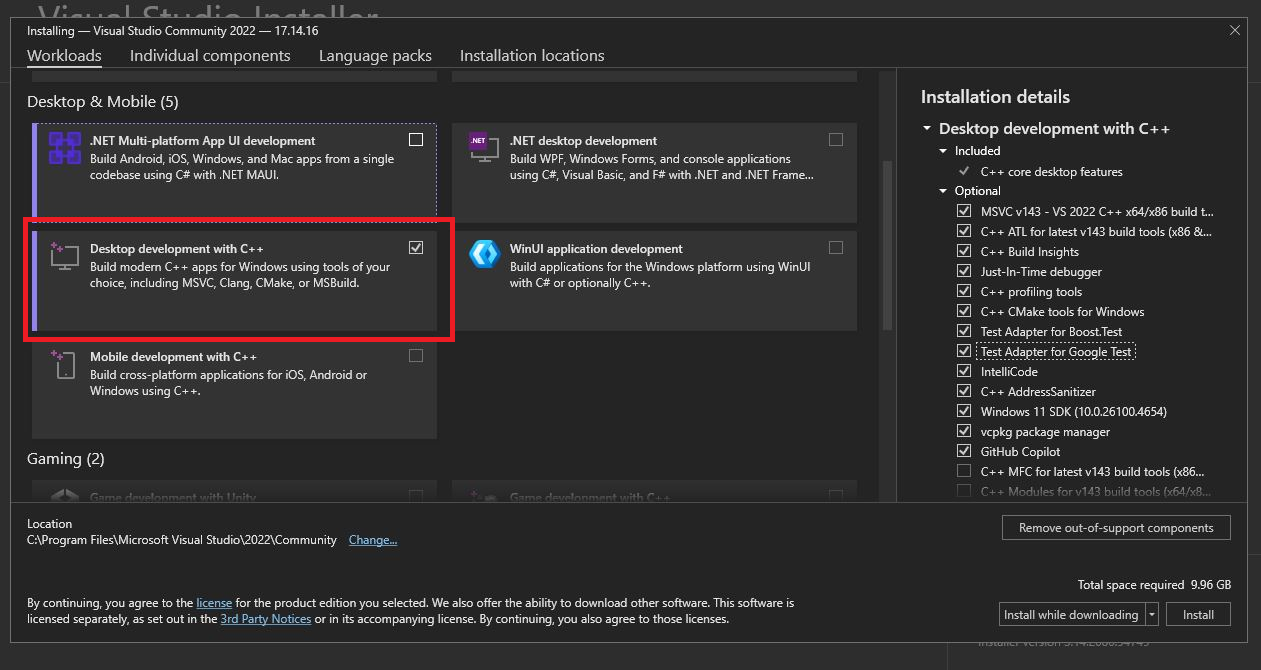
\includegraphics[width=\textwidth]{../Resources/lab0/vs_components.png}

\subsubsection{Utilizare}\label{utilizare}

\begin{enumerate}
\def\labelenumi{\arabic{enumi}.}
\item
    Create project:
%  Creare proiect: \emph{File -\textgreater{} New -\textgreater{} Project\ldots{}}
%\item
%  Tip proiect: \emph{Templates -\textgreater{} Other Languages -\textgreater{} Visual C++ -\textgreater{} Win32 -\textgreater{} Win32 Console App}
\end{enumerate}

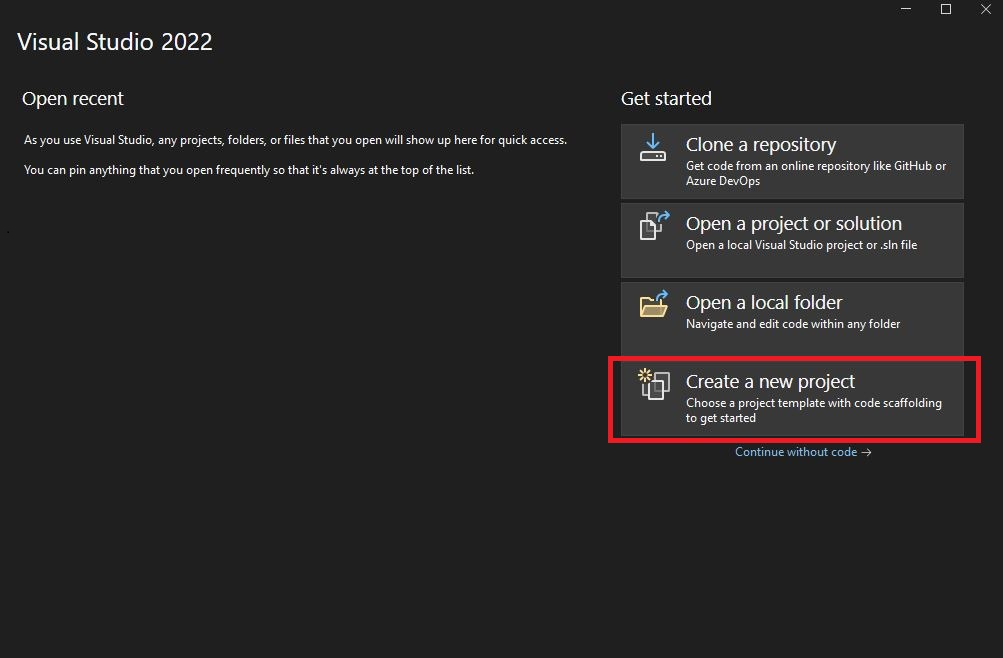
\includegraphics[width=\textwidth]{../Resources/lab0/create_project1.png}

\begin{enumerate}
\def\labelenumi{\arabic{enumi}.}
\setcounter{enumi}{1}
\item
      Select ``\emph{Empty project}''
%Proprietăți proiect: alege ``\emph{Console application}" și bifează ``\emph{Empty project}"
\end{enumerate}

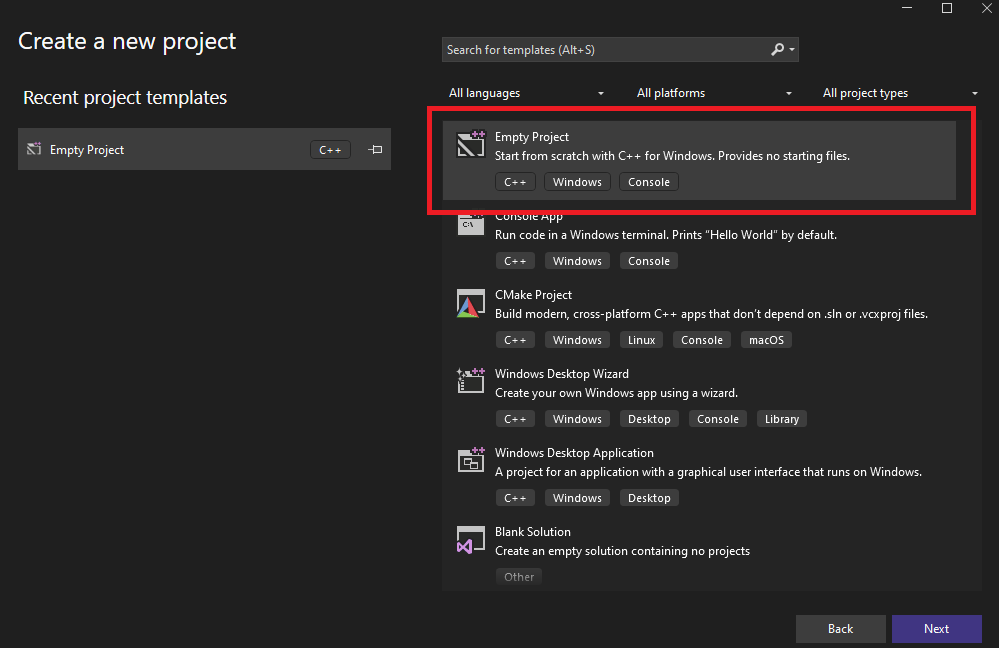
\includegraphics[width=\textwidth]{../Resources/lab0/create_project2.png}
%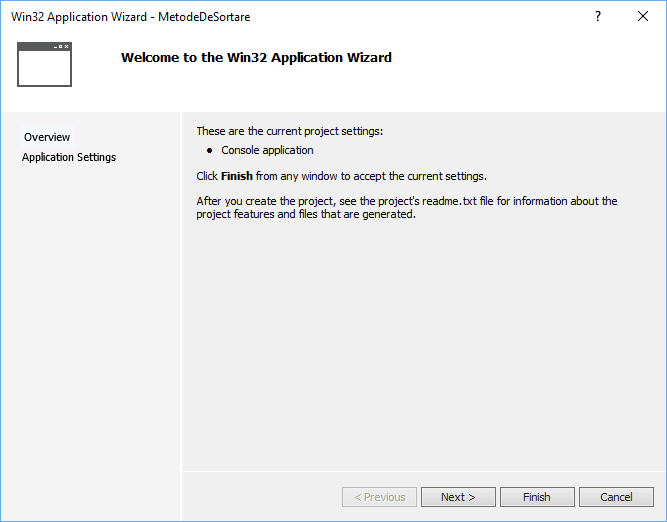
\includegraphics[width=\textwidth]{../Resources/lab0/image2.png}
%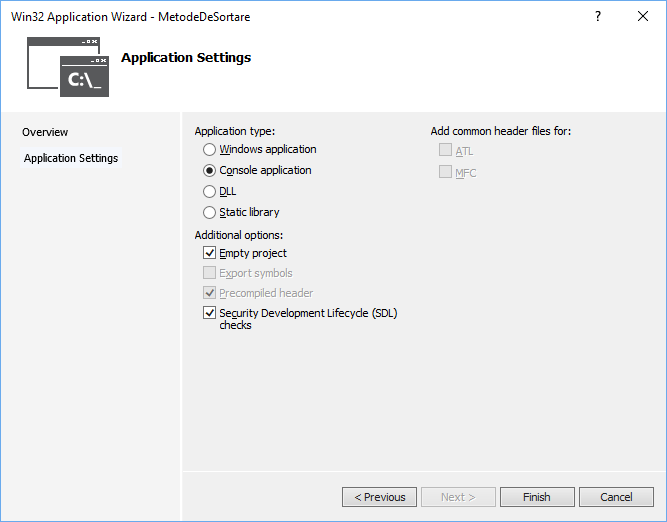
\includegraphics[width=\textwidth]{../Resources/lab0/image3.png}

\begin{enumerate}
\def\labelenumi{\arabic{enumi}.}
\setcounter{enumi}{2}
\item
      Give the project a name.
%Proprietăți proiect: alege ``\emph{Console application}" și bifează ``\emph{Empty project}"
\end{enumerate}

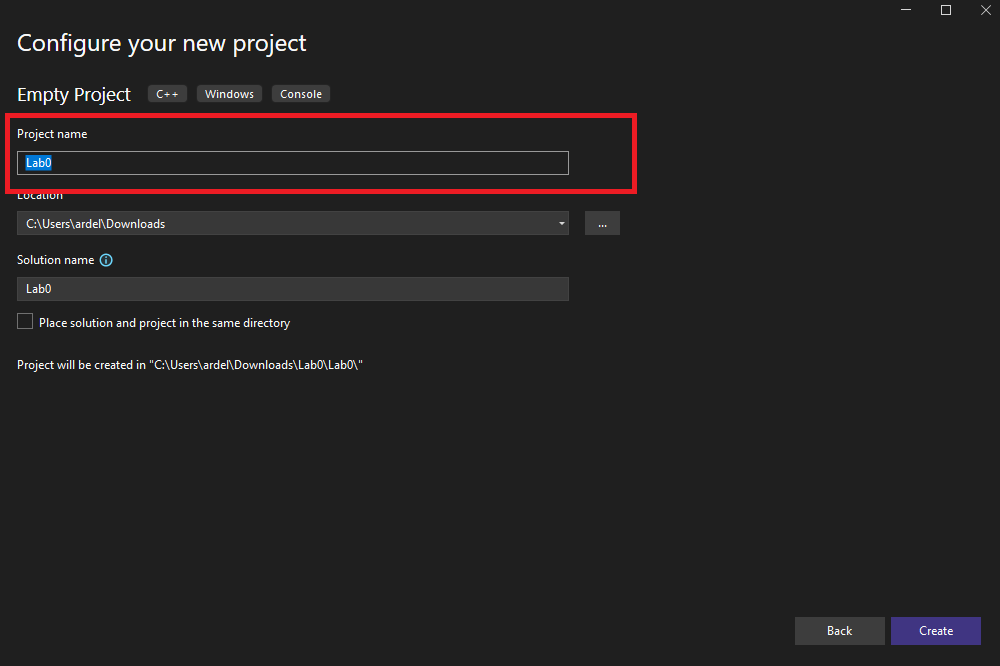
\includegraphics[width=\textwidth]{../Resources/lab0/create_project3.png}

\begin{enumerate}
\def\labelenumi{\arabic{enumi}.}
\setcounter{enumi}{3}
\item
  Creează un fișier \emph{*.cpp} [select from 'Solution Explorer' menu - might be left/right].
\end{enumerate}

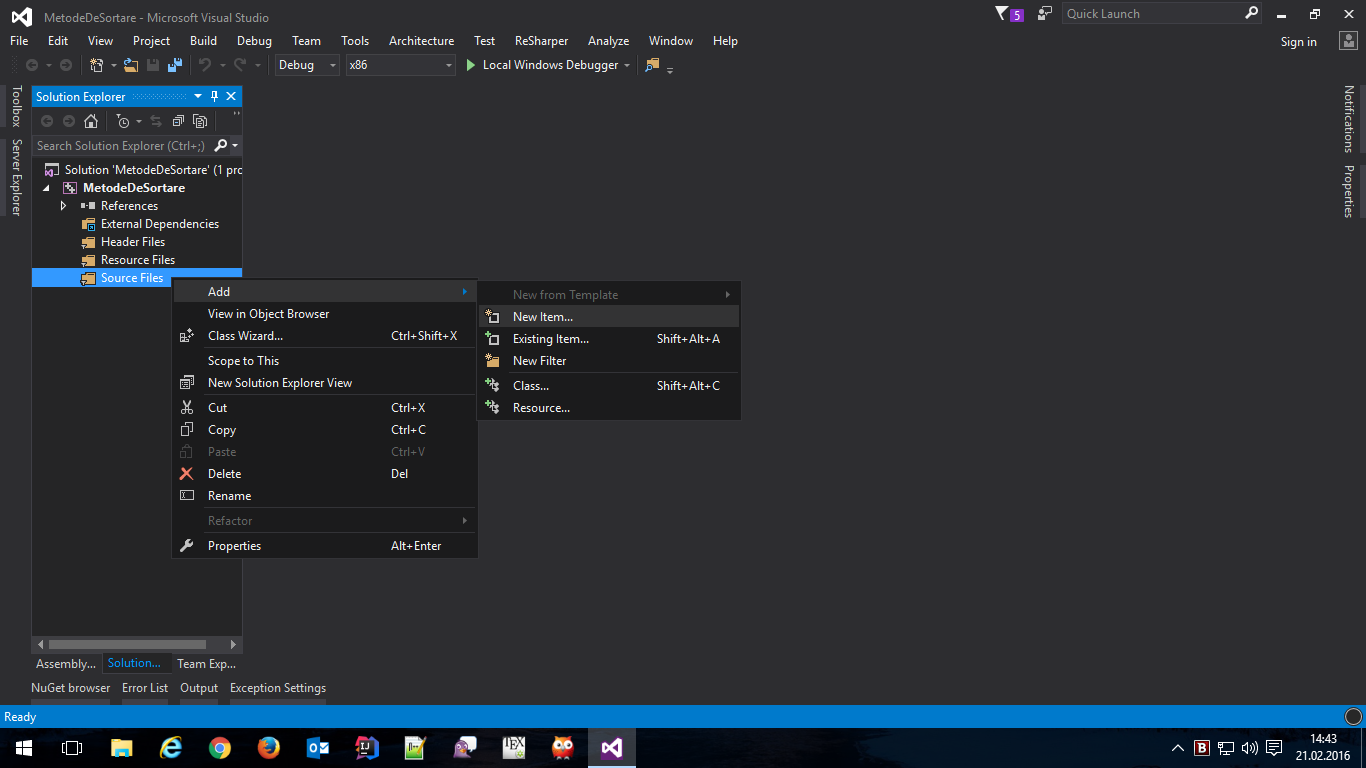
\includegraphics[width=\textwidth]{../Resources/lab0/image4.png}

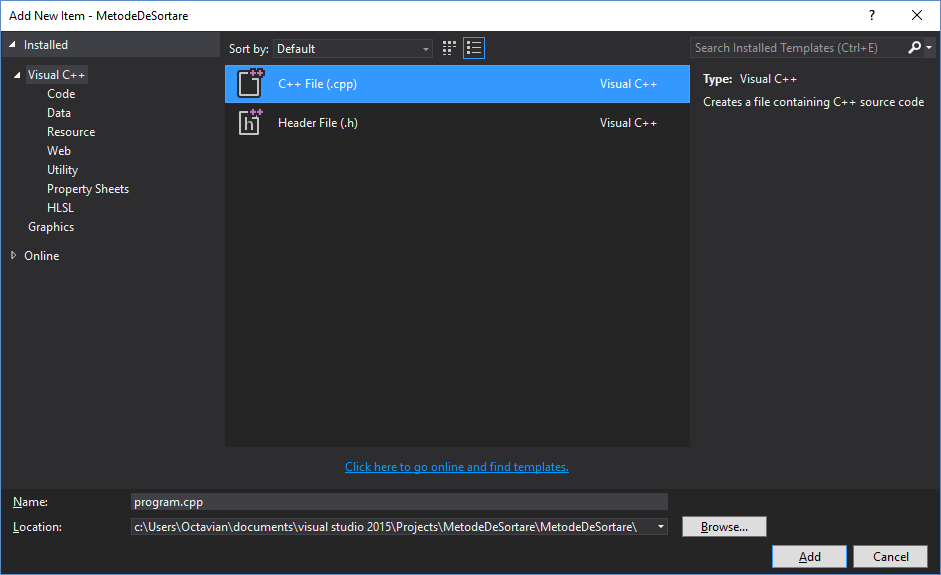
\includegraphics[width=\textwidth]{../Resources/lab0/image5.png}

\begin{enumerate}
\def\labelenumi{\arabic{enumi}.}
\setcounter{enumi}{4}
\item
  Compilare și execuție program (în mod \textbf{DEBUG})
\end{enumerate}

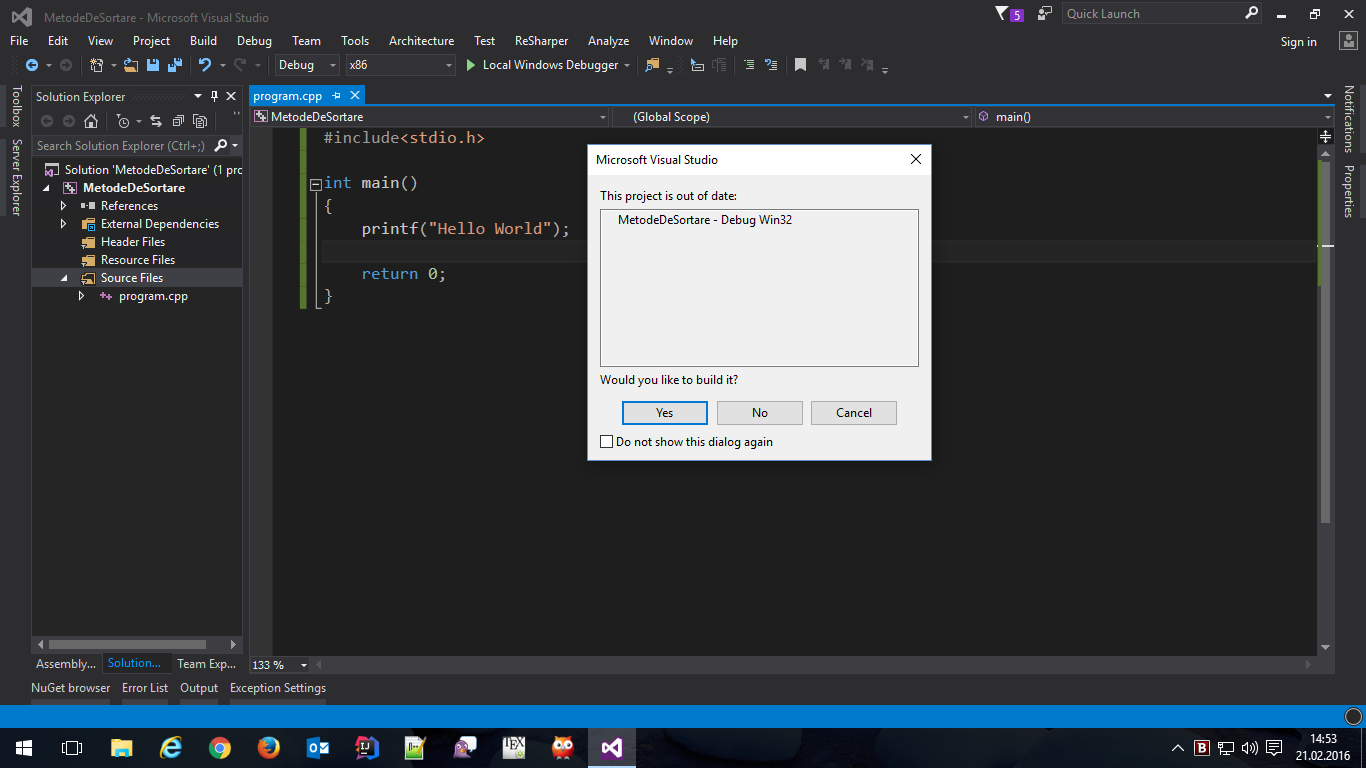
\includegraphics[width=\textwidth]{../Resources/lab0/image6.png}


\subsection{JetBrains CLion}\label{jetbrains-clion}

\subsubsection{Instalare}\label{instalare-1}

Înregistrează-te cu adresa \emph{@student.utcluj.ro} pe
https://www.jetbrains.com/student/

Descarcă și instalează MinGW: https://sourceforge.net/projects/mingw/

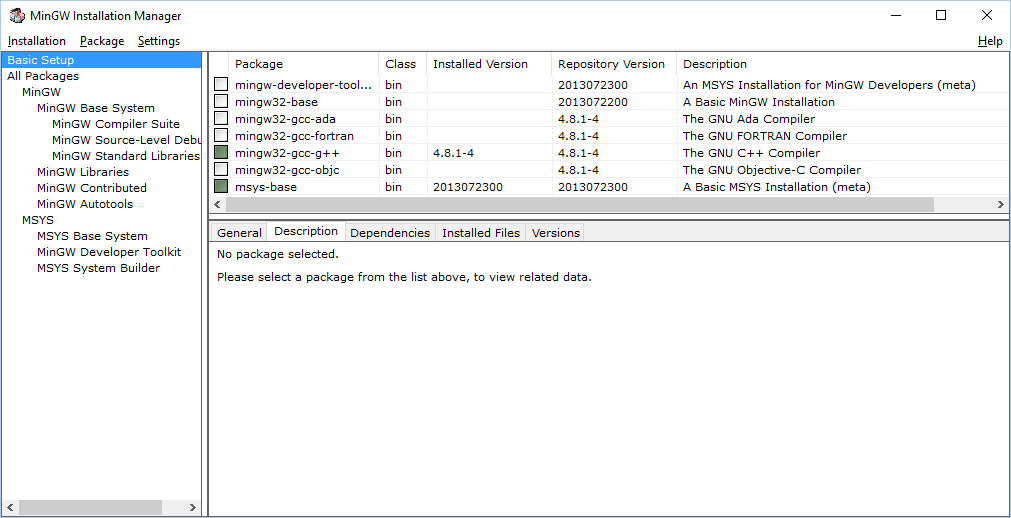
\includegraphics[width=\textwidth]{../Resources/lab0/image7.png}

Descarcă și instalează CLion:
\url{https://www.jetbrains.com/clion/download/\#section=windows}

\subsubsection{Utilizare}\label{utilizare-1}

\begin{enumerate}
\def\labelenumi{\arabic{enumi}.}
\item
  Creare proiect: \emph{New Project}
\end{enumerate}

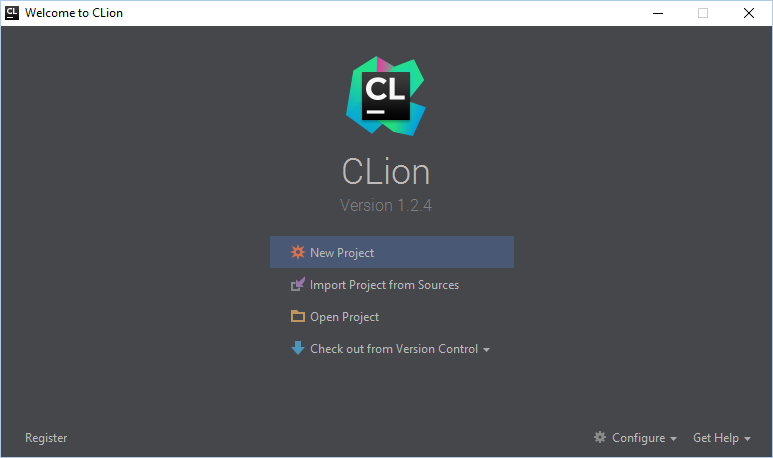
\includegraphics[width=\textwidth]{../Resources/lab0/image8.png}

\begin{enumerate}
\def\labelenumi{\arabic{enumi}.}
\setcounter{enumi}{1}
\item
  Așteaptă până se încarcă simbolurile
\item
  Creează un fișier \emph{*.cpp}
\end{enumerate}

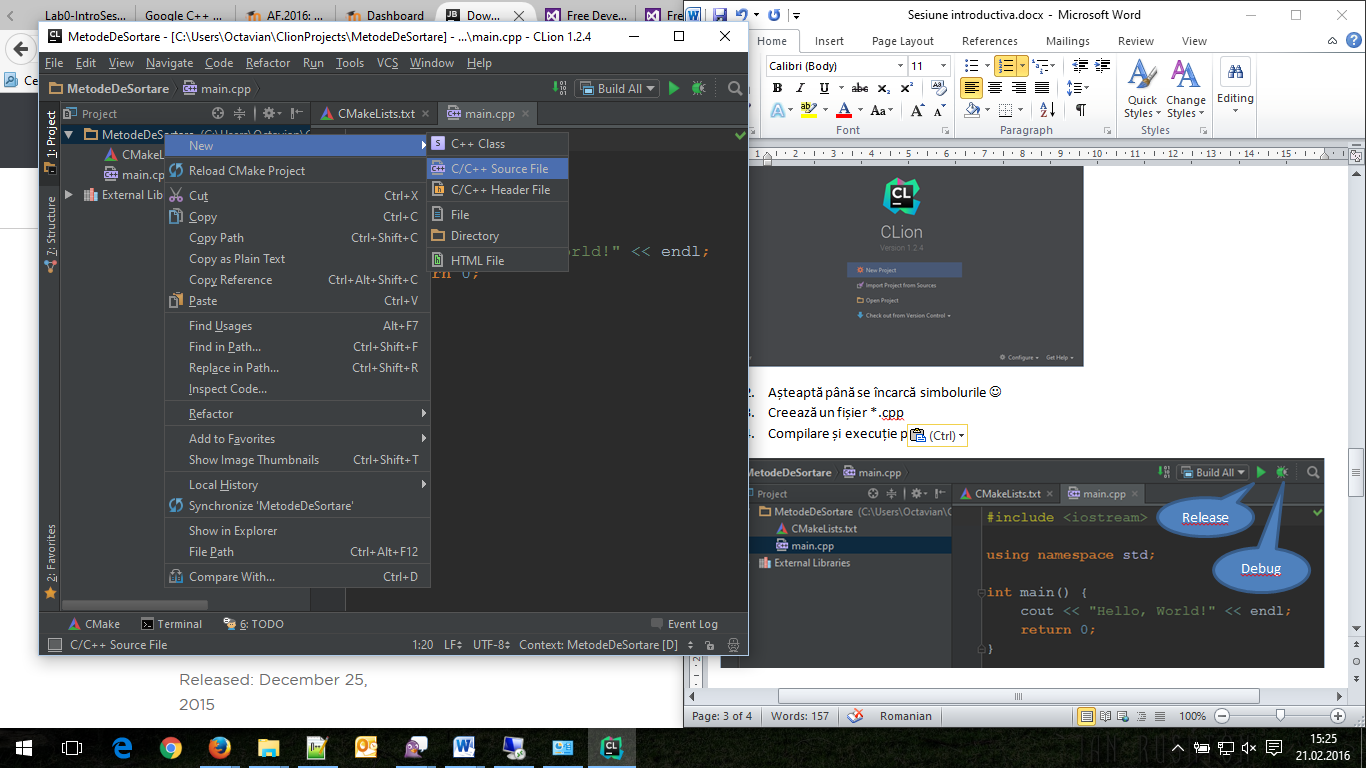
\includegraphics[width=\textwidth]{../Resources/lab0/image9.png}

\begin{enumerate}
\def\labelenumi{\arabic{enumi}.}
\setcounter{enumi}{3}
\item
  Compilare și execuție program
\end{enumerate}

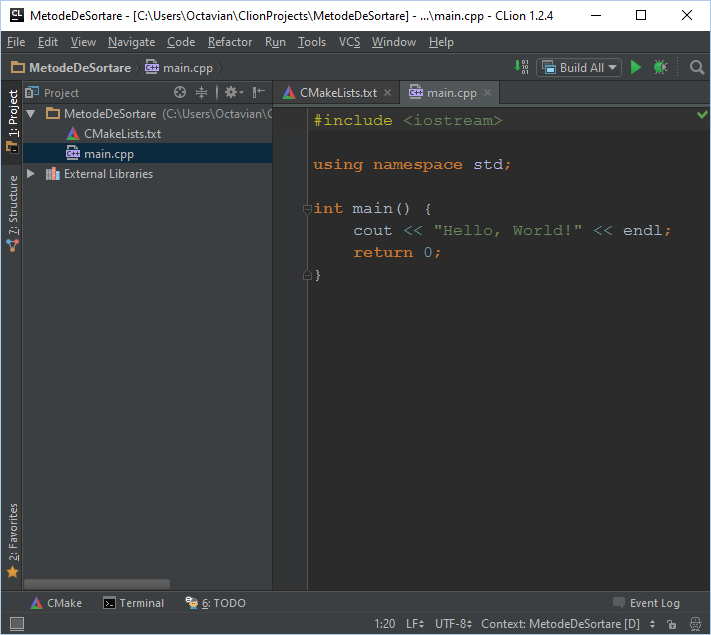
\includegraphics[width=\textwidth]{../Resources/lab0/image10.png}

Debug

Release

\subsection{C/C++}\label{cc}

\subsubsection{Citire/scriere fișiere}\label{citirescriere-fiux219iere}

\textbf{Exercițiu} - pași:

\begin{itemize}
\item
  Declară un sir \emph{v} de lungime \emph{MAX\_SIZE} (o constantă
  definită de tine)
\item
  Citește \emph{n} de la tastatură
\item
  Deschide fișierul \emph{input.txt}, citește \emph{n} numere din el și
  salvează-le în \emph{v}
\item
  Salvează cele \emph{n} numere în fișierul \emph{output.txt} în ordine
  \textbf{inversă}
\end{itemize}

\subsubsection{Generare cazuri de
testare}\label{generare-cazuri-de-testare}

Pentru a testa algoritmii care o să-i implementezi, va trebui să
folosești o serie de date de intrare: șiruri ordonate crescător, șiruri
ordonate descrescător, șiruri aleatoare etc. Generarea șirurilor
crescătoare/descrescătoare ar trebui să fie simplă. Pentru generarea
șirurilor aleatoare poți folosi următoarele:

\begin{itemize}
\item
  Biblioteca \emph{Profiler} de pe Moodle (sau
  \url{https://github.com/cypryoprisa/utcn-fa-profiler})
\end{itemize}

\begin{itemize}
\item
  metodele \emph{rand}(), \emph{srand}(), citește:

  \begin{itemize}
  \item
    \url{http://www.cplusplus.com/reference/cstdlib/rand/}
  \item
    \url{http://www.cplusplus.com/reference/cstdlib/srand/}
  \item
    \url{http://www.cplusplus.com/reference/cstdlib/RAND_MAX/}
  \end{itemize}
\end{itemize}

\textbf{Exercițiu} - pași:

\begin{itemize}
\item
  Citește \emph{n}, \emph{min} și \emph{max} de la tastatură
\item
  Generează un șir aleatoriu de \emph{n} elemente cu valori cuprinse
  intre \emph{min} și \emph{max}
\item
  Șirul trebuie să fie diferit la fiecare rulare a programului
\item
  Adaugă șirul în fișierul \emph{output.txt}
\end{itemize}

\subsubsection{Generare grafice}\label{generare-grafice}

Pentru generarea graficelor poți folosi:

\begin{itemize}
\item
  Biblioteca \emph{Profiler} de pe Moodle (sau
  \url{https://github.com/cypryoprisa/utcn-fa-profiler})
\end{itemize}

\begin{itemize}
\item
  Microsoft Office Excel
\end{itemize}

\subsubsection{Microsoft Office Excel}\label{microsoft-office-excel}

Va trebui să creezi un fișier cu extensia \emph{.csv} (comma-separated
values). Fișierul ar trebui să aibă o structură de felul următor:\\\\

n,asignari\_f1,comparatii\_f1,asignari\_m2,comparatii\_m2

100,1146,1228,1168,1268

200,2634,2820,2678,2878

300,4360,4635,4442,4742

400,6172,6520,6212,6612

500,8042,8458,8090,8590
\\\\
Legendă:

\begin{itemize}
\item
  n=dimensiunea problemei (ex: lungimea șirului de intrare)
\item
  asignari\_f1=numărul de asignări pentru cazul favorabil și metoda 1
\item
  comparatii\_f2=numărul de comparații pentru cazul favorabil și metoda
  2
\end{itemize}

\textbf{Atenție}: Dacă deschizi fișierul CSV în Excel și valorile apar
pe o singura coloană înseamnă că trebuie să folosești alt caracter de
separare (ex: folosește punct și virgulă ";").

După ce ai deschis fișierul CSV în Excel, selectează toate valorile și
creează un \emph{PivotChart}.

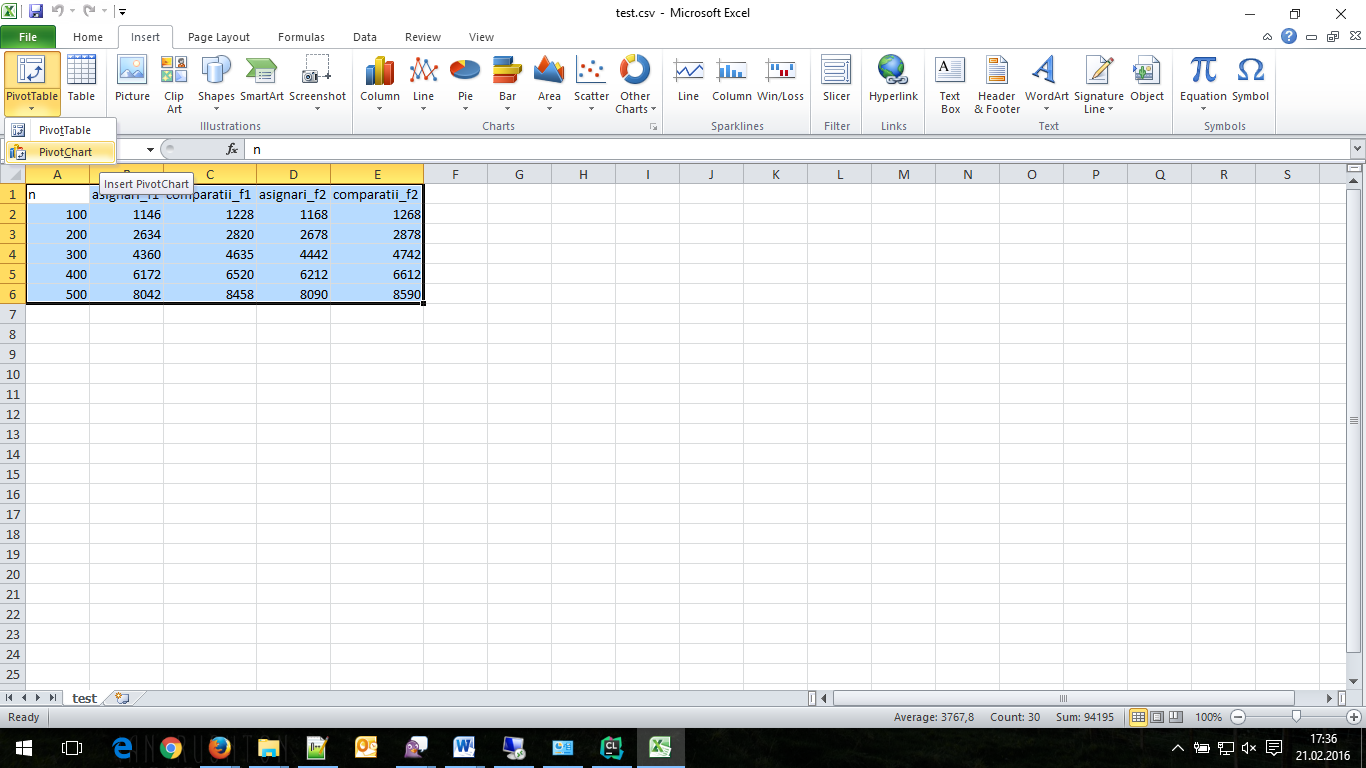
\includegraphics[width=\textwidth]{../Resources/lab0/image11.png}

După ce apeși pe \emph{Ok}", fereastra ar trebui să arate ca în poza de
mai jos.

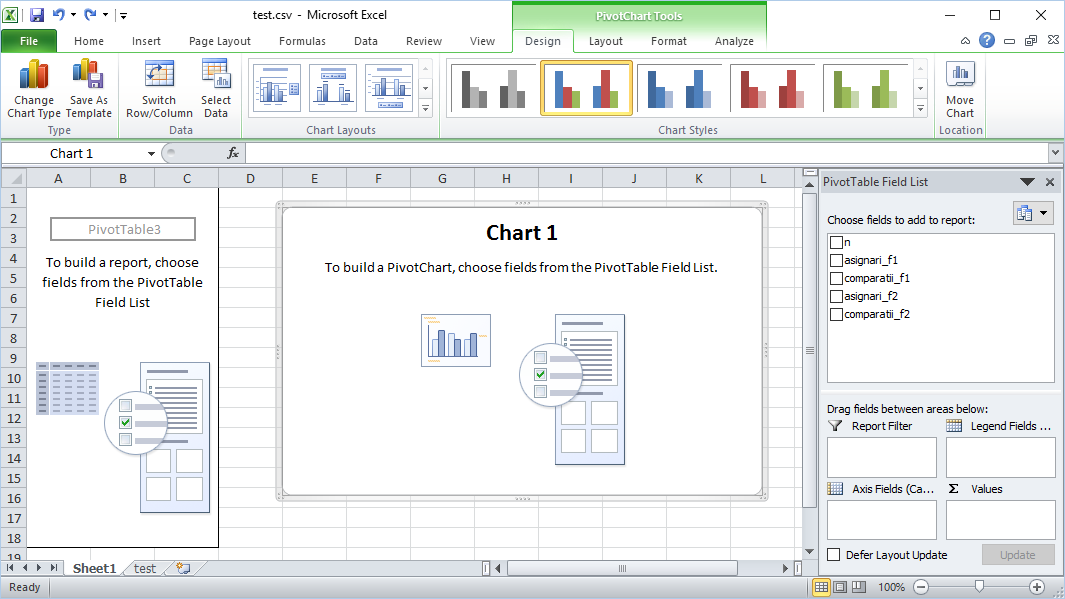
\includegraphics[width=4.5019in,height=2.5319in]{../Resources/lab0/image12.png}

În panoul din stânga trage "\emph{n}" în zona "\emph{Axis Fields}" și
celelalte coloane în zona "\emph{Values}".

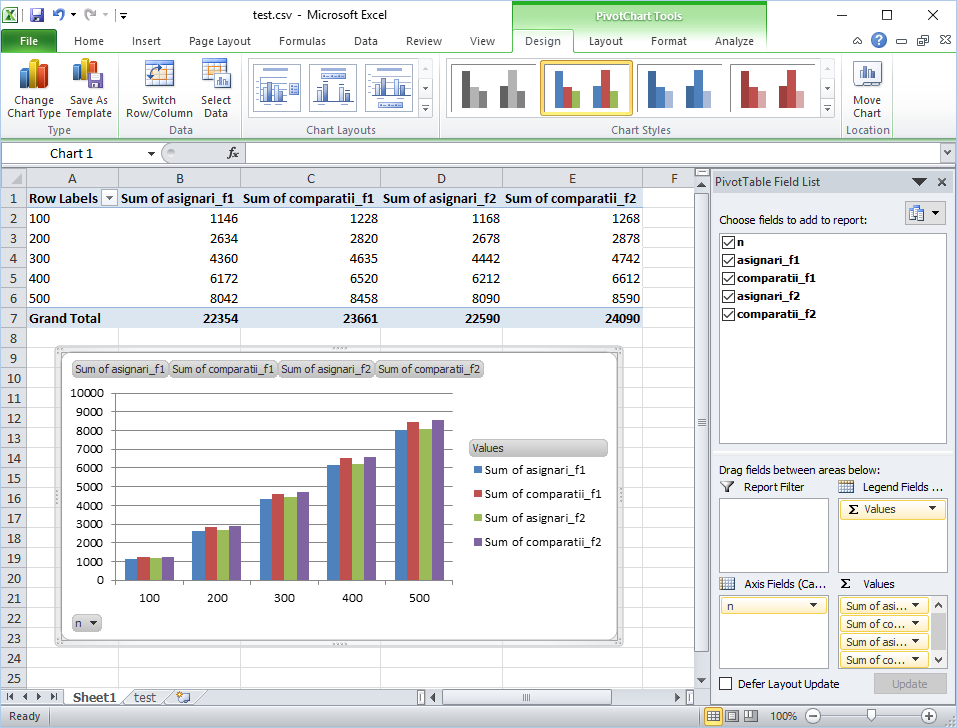
\includegraphics[width=\textwidth]{../Resources/lab0/image13.png}

Schimbă funcția de agregare "\emph{sum}" în "\emph{average}": click pe
săgeata neagra de la fiecare rând din zona "\emph{Values}", apoi
"\emph{Value Field Settings}" și alege "\emph{Average}". Dacă le-ai
schimbat corect, fereastra ar trebui să arate ca în poza de mai jos.

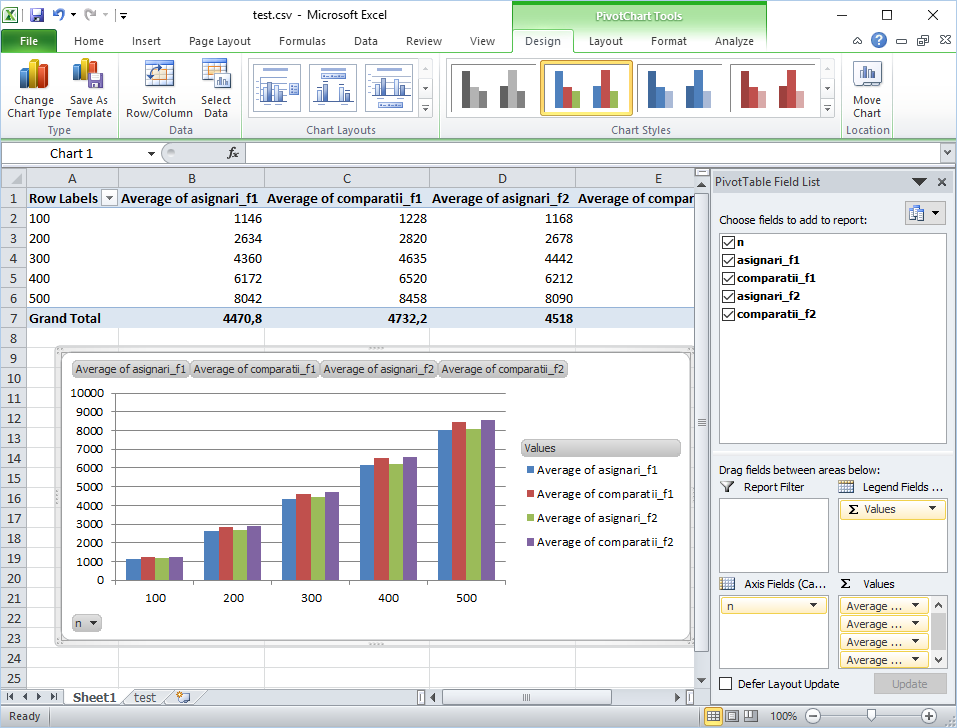
\includegraphics[width=4.29645in,height=3.26824in]{../Resources/lab0/image14.png}

Ultimul pas este să schimbi tipul graficului intr-un grafic de tip linie
de la "\emph{Change Chart Type}". Rezultatul final ar trebui să arate
așa:

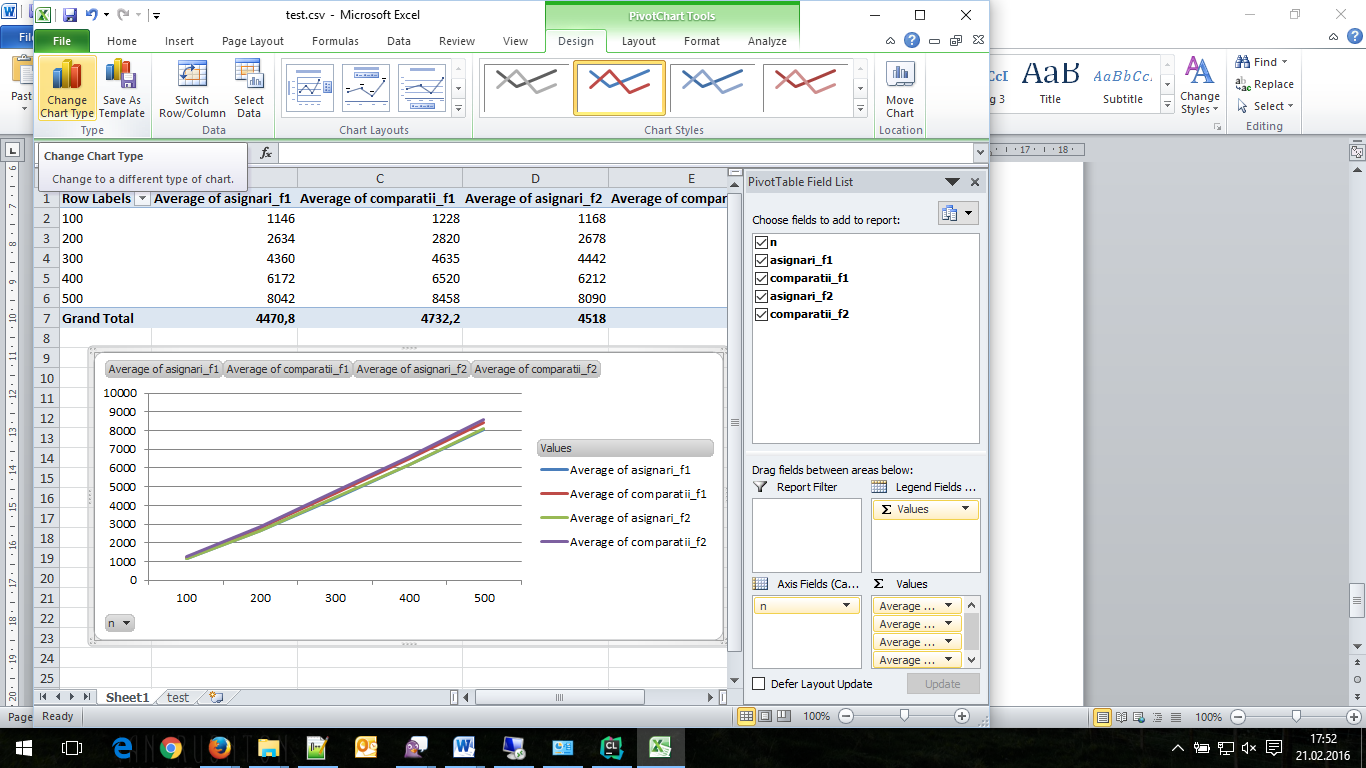
\includegraphics[width=\textwidth]{../Resources/lab0/image15.png}

\subsubsection{Exercițiu}\label{exerciux21biu}

Scrie un program care pentru fiecare \emph{n} din intervalul \{100, 200,
\ldots, 10.000\} calculează și adaugă într-un fișier următoarele valori:

n, 100*log(n), 10*n, n*log(n), 0.1*n\textsuperscript{2},
0.01*n\textsuperscript{3}

Folosește valorile din fișier ca să generezi un grafic în funcție de
\emph{n}.

\end{document}